\documentclass[journal,compsoc]{IEEEtran}
% Some/most Computer Society conferences require the compsoc mode option,
% but others may want the standard conference format.
%
% If IEEEtran.cls has not been installed into the LaTeX system files,
% manually specify the path to it like:
% \documentclass[conference,compsoc]{../sty/IEEEtran}

% *** CITATION PACKAGES ***
%
\ifCLASSOPTIONcompsoc
  % IEEE Computer Society needs nocompress option
  % requires cite.sty v4.0 or later (November 2003)
  \usepackage[nocompress]{cite}
\else
  % normal IEEE
  \usepackage{cite}
\fi

% *** GRAPHICS RELATED PACKAGES ***
%
\ifCLASSINFOpdf
  % \usepackage[pdftex]{graphicx}
  % declare the path(s) where your graphic files are
  % \graphicspath{{../pdf/}{../jpeg/}}
  % and their extensions so you won't have to specify these with
  % every instance of \includegraphics
  % \DeclareGraphicsExtensions{.pdf,.jpeg,.png}
\else
  % or other class option (dvipsone, dvipdf, if not using dvips). graphicx
  % will default to the driver specified in the system graphics.cfg if no
  % driver is specified.
  % \usepackage[dvips]{graphicx}
  % declare the path(s) where your graphic files are
  % \graphicspath{{../eps/}}
  % and their extensions so you won't have to specify these with
  % every instance of \includegraphics
  % \DeclareGraphicsExtensions{.eps}
\fi

% correct bad hyphenation here
\hyphenation{op-tical net-works semi-conduc-tor}

\usepackage{graphicx}
\graphicspath{{figures/}}

\begin{document}
\bstctlcite{IEEEexample:BSTcontrol}
%
% paper title
% Titles are generally capitalized except for words such as a, an, and, as,
% at, but, by, for, in, nor, of, on, or, the, to and up, which are usually
% not capitalized unless they are the first or last word of the title.
% Linebreaks \\ can be used within to get better formatting as desired.
% Do not put math or special symbols in the title.
\title{Machine Learning for Automated Diagnosis of Skin Lesions}


% author names and affiliations
% use a multiple column layout for up to three different
% affiliations
\author{
\IEEEauthorblockN{Fábio Santos, Email: fmts@ua.pt} \par
\IEEEauthorblockA{Supervisors: Filipe Silva, Pétia Georgieva \\
Department of Electronics Telecomunications and Informatics\\
University of Aveiro, Aveiro, 3810-193\\
}
}

% conference papers do not typically use \thanks and this command
% is locked out in conference mode. If really needed, such as for
% the acknowledgment of grants, issue a \IEEEoverridecommandlockouts
% after \documentclass

% for over three affiliations, or if they all won't fit within the width
% of the page (and note that there is less available width in this regard for
% compsoc conferences compared to traditional conferences), use this
% alternative format:
% 
%\author{\IEEEauthorblockN{Michael Shell\IEEEauthorrefmark{1},
%Homer Simpson\IEEEauthorrefmark{2},
%James Kirk\IEEEauthorrefmark{3}, 
%Montgomery Scott\IEEEauthorrefmark{3} and
%Eldon Tyrell\IEEEauthorrefmark{4}}
%\IEEEauthorblockA{\IEEEauthorrefmark{1}School of Electrical and Computer Engineering\\
%Georgia Institute of Technology,
%Atlanta, Georgia 30332--0250\\ Email: see http://www.michaelshell.org/contact.html}
%\IEEEauthorblockA{\IEEEauthorrefmark{2}Twentieth Century Fox, Springfield, USA\\
%Email: homer@thesimpsons.com}
%\IEEEauthorblockA{\IEEEauthorrefmark{3}Starfleet Academy, San Francisco, California 96678-2391\\
%Telephone: (800) 555--1212, Fax: (888) 555--1212}
%\IEEEauthorblockA{\IEEEauthorrefmark{4}Tyrell Inc., 123 Replicant Street, Los Angeles, California 90210--4321}}




% use for special paper notices
%\IEEEspecialpapernotice{(Invited Paper)}




% make the title area
\maketitle

% As a general rule, do not put math, special symbols or citations
% in the abstract
\begin{abstract}
Machine learning, specifically, deep learning is a fast-growing field that is being used for multiple medical imaging related problems, such as early detection of skin cancer. For a long time, automated diagnosis of skin cancer from clinical images was considered to be out of reach. However, recent works based on deep networks produced promising results which have the potential to change the landscape of skin lesion diagnosis. Systems created based on these new advancements aim to  provide support for both dermatologists in the decision making process and for patients that do not have access to skin professionals.  
This paper focuses on the current state of automated skin lesion diagnosis using convolutional neural network models, while also providing a comprehensive look into the requirements of integrating such models into a web application capable of helping dermatologists on the diagnosis of skin lesions.
\end{abstract}

\begin{IEEEkeywords} Automatic assessment tools, eHealth, machine learning, medical imaging \end{IEEEkeywords}

% For peer review papers, you can put extra information on the cover
% page as needed:
% \ifCLASSOPTIONpeerreview
% \begin{center} \bfseries EDICS Category: 3-BBND \end{center}
% \fi
%
% For peerreview papers, this IEEEtran command inserts a page break and
% creates the second title. It will be ignored for other modes.
\IEEEpeerreviewmaketitle

\section{Introduction}
\subsection{Background}
Skin cancer is the most common type of cancer, particularly, in the United States of America the incidence rates keep rising with currently 1 in 5 persons developing skin cancer until the age of 70 \cite{Foundation2019}. However, skin cancer represents a problem not only for America but also for the international health community in general. For example, in Europe, over 100000 people are diagnosed with melanoma and 22000 deaths annually occur due to this form of skin cancer \cite{Bray2018}.  Yet, one of the most remarkable facts about skin cancer is that when detected on late stages there is a 23\% chance of survival, but when detected early the 5 year survival rate rises to 99\% \cite{Foundation2019}. Therefore, the early detection of skin cancer is an absolute priority. \par
Skin cancer can be detected by dermatology professionals by simple visual examination of skin lesions. However, the difference between malignant and benign skin lesions can be negligible making it a difficult task even for trained medical experts. As such, a medical application which provides automated skin lesion diagnosis for decision support is an welcome addition to this field. \par
Initially, automated diagnosis of skin lesions was made based on predefined techniques well known by dermatology professionals such as the ABCDE rule (Asymmetry, Border, Color, Dermoscopic structure and Evolving), but often failed to either generalize to new cases or lacked the accuracy of a human. However, in more recent years, machine learning approaches into skin lesion diagnosis shows remarkable performance in comparison with the hand crafted algorithms, specially with deep learning methods\cite{Esteva2017}\cite{Haenssle2018}. 
\subsection{Objectives and Motivation}
A strong assumption can be made that if an accurate automated skin lesion diagnosis tool is used by dermatologists, then skin cancer cases will be detected earlier. Therefore, the main objective behind this dissertation is to improve the current work on automated skin lesion diagnosis by using deep learning techniques. This work will be part of a tool that has the intent of being used in a clinic context, so the priority is to its performance as much as possible. \par 
Finally, the aforementioned tool must be packaged within a eHealth application, in order to be easily accessed by medical professionals in a clinical environment. Such application must have the ability to potentially integrate other components useful for both dermatologists and patients while enabling easy communication between them. 
\section{Literature review}
The following sections are structured as follows. Section 2.1 provides an exploratory look into eHealth/mHealth applications for skin lesion diagnosis. Section 2.2 gives an overview of deep learning applied into medical imaging. Finally, Section 2.3 reviews some of the current approaches towards skin lesion diagnosis systems using deep learning. 
\subsection{eHealth/mHealth for skin lesion diagnosis}
Online health, ehealth and mhealth applications represent a rapidly developing field of medicine that has the potential to become powerful tool in the diagnosis and management of skin diseases \cite{Jaworek-Korjakowska2018}. These applications aim to enhance clinical care, promote health, prevent diseases and most importantly provide medical support when it is not available at a particular location or time. Generally, the acceptance towards this type of systems in the medical community keeps growing, but is highly dependent on factors such as performance, accessibility and ease of use, which poses challenges for their global adoption. \par
Currently, several production ready skin lesion classification systems are  available for both skin professionals and patients wishing to self monitor their own skin. However, almost none of them has shown to be sufficiently accurate or reliable enough for a clinical environment. \par 
One of the most popular eHealth applications for this purpose is Metaoptima's Dermengine web application. Their Visual Search tool compares a user-submitted image with similar images in a database of thousands of pathology-labelled images gathered from  other dermatologists. Deep learning techniques are used to search for related images based on visual features such as colour, shape or patterns \cite{dermengine}. \par
Another popular app is the SkinVision which classifies lesions as either low, medium or high risk of skin cancer by using an risk assessment algorithm based on gray-scale images of lesions and their associated fractal maps. It achieves the overall sensitivity of 73\%, specificity of 83\%, and accuracy of 81\%. The positive and negative predictive values were 49\% and 83\%, respectively \cite{Jaworek-Korjakowska2018}.
\subsection{Deep neural networks for medical imaging}
Deep learning refers to computational models composed of multiple processing layers capable of learning representations of data with multiple levels of abstraction \cite{Goodfellow-et-al-2016}. The initial impact of deep learning for medical imaging was revealed through a special issue published in 2016 at the IEEE Transactions on Medical Imaging \cite{Greenspan2016}. It explains the principles and methods of deep learning applied to medical image analysis. These structures can be found in approaches to medical imaging problems such as organ segmentation, lesion detection and tumor classification. \par
The main advantage of deep learning over other machine learning algorithms is that it removes the need for feature engineering, a process that requires knowledge of the problem domain, which can be a time consuming process as well as introduce human error.\par
Recently, deep neural networks appear as state-of-the-art solutions for medical imaging problems due to advancements in the field. These advancements include the research and development of new methods to prevent overfitting, the rise of computational power along with the use of graphical processing units, and finally the development of high level modules such as theano \cite{Bastien} that help train and test neural networks . 
\subsection{Skin lesion classification using deep learning}
One of the most important factors which determines the performance of a deep learning model is the dataset used to train it on. For general image recognition problems datasets such as ImageNet \cite{Deng2010} which contains over 14 Million samples with over 20000 classes are usually used and serve as a benchmark. However for skin lesion diagnosis systems, it is difficult and in many times impossible to compare the performance of published classification results since many authors use nonpublic datasets for training and testing \cite{Brinker2018}. The closest benchmark available for this domain is the HAM10000 dataset \cite{ham10000}. \par
Nonetheless, organizations such as International Skin Imaging Collaboration (ISIC) provide an open source public access archives of skin images, which can be used for teaching or for the development and testing of automated skin lesion diagnosis systems \cite{isic2019}. They also place a challenge around their dataset every year in order to improve the performance of this classification systems as a whole. \par
\subsubsection{Transfer learning approaches}
The most popular approach for skin cancer classification using deep learning, specifically, convolutional neural networks, was published in 2017 by Esteva et al.\cite{Esteva2017} and could diagnose keratinocyte and melanoma cancer. The authors follow a transfer learning approach by leveraging the weights of the InceptionV3 network trained on ImageNet, on top of which they build their own classifier. Finally, they measured the network's performance by pitting it against 21 dermatologists and concluded that their classifier had comparable performance to that of those board-certified dermatologists. This network used a very large set of labelled images in order to achieve high accuracy, namely, 129450 clinical images. This data was a combination of multiple sources, both proprietary and publicly available. \par
In the meantime, submissions to ISIC challenges have also been trying new concepts that improve the skin lesion diagnosis model's performance. In the part 3 of the ISIC 2018 challenge participants were asked to develop a classifier to distinguish between 7 different types of skin cancer and the ranking was made based on their normalized multiclass accuracy \cite{isic2018}. The top 3 submissions had balanced accuracies of about 88,5\%, 88,2\%, 87,1\% respectively and were all submited by Metaoptima (the company behind Dermengine) \cite{isic2018top3}. To train those models they used the provided dataset along with proprietary data. Additionally, they augmented the training data by performing random horizontal flips, random rotations, changes in brightness, saturation, and contrast. They used transfer learning from several pre trained models trained on ImageNet (such as InceptionV3 or ResNet) and then ensembled the best performing ones \cite{isic2018top3}. \par
The 2019's version of this challenge asked participants to classify dermoscopic images among nine different diagnostic categories, however this time around one of the classes was "unknown" (none of the others). Similarly to the 2018's version participants could use their own data to improve the network's performance and were ranked based on a balanced multiclass accuracy \cite{isic2019}. The results turned out to be quite promising, with the best submission posted by Geesert et al. \cite{isic2019first} scoring 92.6\% accuracy. They trained their networks on a combination of multiple datasets that also included the HAM10000 \cite{ham10000}. \par
Gessert's et al. approach to preprocessing was to first crop the images, perform image binarization, apply the shades of gray color constancy method and finally resize the images. Data augmentation is also applied by randomly changing brightness, contrast, rotation, scale, shear and flip. They used two different input strategies, the first takes a random crop from the preprocessed image, the second randomly resizes and scales the image when taking a crop from the preprocessed one. Like the previous attempts they use a transfer learning approach relying on EfficientNets that were trained on the ImageNet dataset. For each model, predictions for each model are made based on which input strategy was used. The final prediction is made using an ensemble of a subset which contained all the best performing models.
\subsubsection{End to end learning approaches}
The most common approach to skin lesion classification is through transfer learning. However, end to end learning can make sense in specific contexts. For instance, when data and computational resources is not scarce. \par 
In 2019, Ly et al. \cite{Ly2019}, trained multiple models from scratch with the intention of deploying such models for offline usage in smartphones. They justified this decision by arguing that using pre trained models with large neural network architectures requires a lot more parameters than models trained from scratch. Their best model attained 86\% accuracy, significantly better than other transfer learning approaches, while being much more compact (29M). However, they used a huge dataset titled "PHDB" which was composed of multiple other datasets and contained 80,192 labeled images, which explains the high performance.
% An example of a floating figure using the graphicx package.
% Note that \label must occur AFTER (or within) \caption.
% For figures, \caption should occur after the \includegraphics.
% Note that IEEEtran v1.7 and later has special internal code that
% is designed to preserve the operation of \label within \caption
% even when the captionsoff option is in effect. However, because
% of issues like this, it may be the safest practice to put all your
% \label just after \caption rather than within \caption{}.
%
% Reminder: the "draftcls" or "draftclsnofoot", not "draft", class
% option should be used if it is desired that the figures are to be
% displayed while in draft mode.
%
%\begin{figure}[!t]
%\centering
%\includegraphics[width=2.5in]{myfigure}
% where an .eps filename suffix will be assumed under latex, 
% and a .pdf suffix will be assumed for pdflatex; or what has been declared
% via \DeclareGraphicsExtensions.
%\caption{Simulation results for the network.}
%\label{fig_sim}
%\end{figure}

% Note that the IEEE typically puts floats only at the top, even when this
% results in a large percentage of a column being occupied by floats.


% An example of a double column floating figure using two subfigures.
% (The subfig.sty package must be loaded for this to work.)
% The subfigure \label commands are set within each subfloat command,
% and the \label for the overall figure must come after \caption.
% \hfil is used as a separator to get equal spacing.
% Watch out that the combined width of all the subfigures on a 
% line do not exceed the text width or a line break will occur.
%
%\begin{figure*}[!t]
%\centering
%\subfloat[Case I]{\includegraphics[width=2.5in]{box}%
%\label{fig_first_case}}
%\hfil
%\subfloat[Case II]{\includegraphics[width=2.5in]{box}%
%\label{fig_second_case}}
%\caption{Simulation results for the network.}
%\label{fig_sim}
%\end{figure*}
%
% Note that often IEEE papers with subfigures do not employ subfigure
% captions (using the optional argument to \subfloat[]), but instead will
% reference/describe all of them (a), (b), etc., within the main caption.
% Be aware that for subfig.sty to generate the (a), (b), etc., subfigure
% labels, the optional argument to \subfloat must be present. If a
% subcaption is not desired, just leave its contents blank,
% e.g., \subfloat[].


% An example of a floating table. Note that, for IEEE style tables, the
% \caption command should come BEFORE the table and, given that table
% captions serve much like titles, are usually capitalized except for words
% such as a, an, and, as, at, but, by, for, in, nor, of, on, or, the, to
% and up, which are usually not capitalized unless they are the first or
% last word of the caption. Table text will default to \footnotesize as
% the IEEE normally uses this smaller font for tables.
% The \label must come after \caption as always.
%
%\begin{table}[!t]
%% increase table row spacing, adjust to taste
%\renewcommand{\arraystretch}{1.3}
% if using array.sty, it might be a good idea to tweak the value of
% \extrarowheight as needed to properly center the text within the cells
%\caption{An Example of a Table}
%\label{table_example}
%\centering
%% Some packages, such as MDW tools, offer better commands for making tables
%% than the plain LaTeX2e tabular which is used here.
%\begin{tabular}{|c||c|}
%\hline
%One & Two\\
%\hline
%Three & Four\\
%\hline
%\end{tabular}
%\end{table}


% Note that the IEEE does not put floats in the very first column
% - or typically anywhere on the first page for that matter. Also,
% in-text middle ("here") positioning is typically not used, but it
% is allowed and encouraged for Computer Society conferences (but
% not Computer Society journals). Most IEEE journals/conferences use
% top floats exclusively. 
% Note that, LaTeX2e, unlike IEEE journals/conferences, places
% footnotes above bottom floats. This can be corrected via the
% \fnbelowfloat command of the stfloats package.


\section{Methods and materials}
The following sections are structured as follows. Section 3.1 provides an explanatory view into the most used image recognition neural network typology. Section 3.2 describes two of the most popular CNN architectures. Section 3.3 explores the concept of repurposing pre-trained models from CNN architectures trained on generic datasets. Section 3.4 explores problems related to training deep networks and some solutions. Finally, Section 3.5 explores state of the art frameworks for training and deploying deep networks.   
\subsection{Convolutional neural networks}
Artificial Neural Networks (ANNs) compose a category of machine learning algorithms that are inspired by biological neural networks. These structures are composed by multiple layers, each composed by multiple neurons that can be interpreted as a function described by parameters. We can look at ANNs as an iterative process that tries to optimize parameters in order to minimize a cost function. \par
ANNs can approximate any function with few layers, but for more complex problems it deviates a lot from true predictions. Therefore, networks with many more layers and with an organization which allows them to create levels of abstraction are often used to solve more complex problems. We call such networks deep neural networks. \par
There are many different typologies of ANNs. The most common has a fully connected structure between layers, where each neuron is connected to every other neuron in the previous layer. However, in image recognition such network architecture does not take into account the spatial structure of images. For example, it treats input pixels which are far apart and close together on exactly the same footing. \par
Instead, convolutional neural networks (CNN) or some close variant are used in most neural networks for image recognition problems\cite{Nielsen2017a}. They still retain the core concepts of ANNs, but add 3 different concepts which distinguish them from conventional ANNs:
\begin{itemize}
\item Local receptive fields: Each neuron in the first hidden layer will be connected only to a small region of the input neurons.
\item Shared weights: Weights and biases are shared across the hidden neurons so that convolutional networks become well adapted to translation variances in images. The shared weights are often said to define a kernel or filter, while to the map from the input layer to the hidden layer we call feature map, where a feature detected by a hidden neuron is some kind of input pattern that will cause the neuron to activate. To do image recognition we need multiple feature maps in order to recognize multiple features.
\item Pooling layers: These layers simplify the information in the output from the convolutional layer by removing unnecessary information, such as noise. A common pool layer is max pooling which provides a way to know if a given feature is found anywhere in a region of a image \cite{Nielsen2017a}.
\end{itemize}
\subsection{Convolutional neural network architectures}
Over the years several CNN architectures have been developed and tested against state of the art benchmark challenges such as the Imagenet Large Scale Visual Recognition Challenge (ILSVRC) \cite{ilsvrc}. In 2012, Krizhevsky et al. \cite{alexnet} submited for the first time a CNN architecture (AlexNet) which outperformed hand-crafted feature learning on the ImageNet. It contained 8 neural network layers, 5 convolutional and 3 fully-connected. This laid the foundation for traditional CNNs: a convolutional layer followed by an activation function followed by a max pooling operation. \par
Following AlexNet main ideas, the VGGNet\cite{vggnet} was created and became quite popular by winning the 2014’s ILSVR. This architecture proved that representation depth is beneficial for the classification accuracy, by using the traditional convolutional network architecture but with increased depth along with smaller receptive fields. There are some public variations of this network, one of which having 16 weight layers (VGG16) displayed in Fig. 1. This architecture is composed by multiple sets of convolutional layers followed by pooling layers that build progressively more abstract features, and at the end a fully connected structure to convert the results of the convolution into a label.
\begin{figure}[ht]
  \centering
    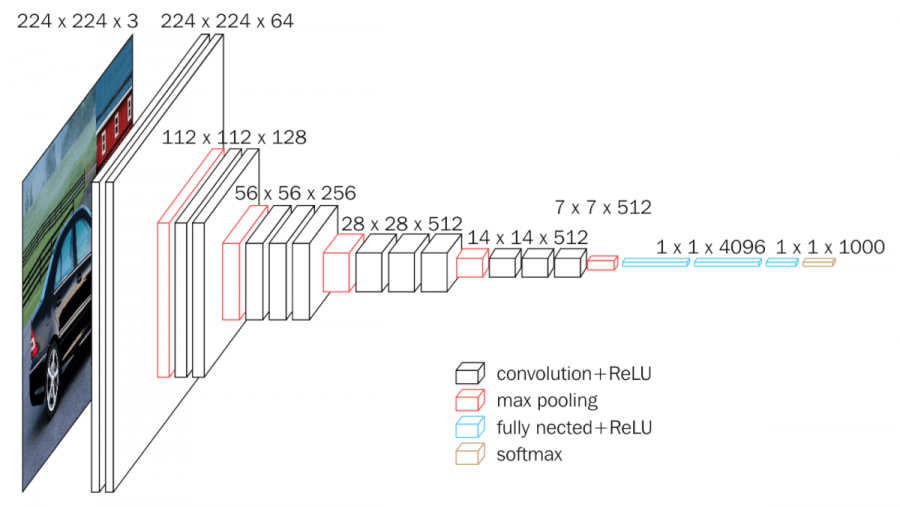
\includegraphics[scale=0.5, width=\linewidth]{figures/vgg16.png}
  \caption{Architecture of the VGG16 convolutional neural network \cite{vggnet}}
\end{figure}
\subsection{Transfer learning}
Supervised learning using deep neural networks requires large amounts of data and computational power in order to train models. However, both of which can either be impossible to have or quite difficult to acquire for small teams. However, even when one has a good dataset along with high computational power, the training process can take a long time, especially while debugging the network to determine a good model fit. \par
As such, transfer learning techniques are usually used to solve image classification problems \cite{Ly2019}, which is a common concept used to minimize the effects of the aforementioned problems. Transfer learning is a method of reusing a pre trained model's knowledge for another related task\cite{DipanjanSarkarRaghavBali2018}. In deep learning, using transfer learning means to carry the parameters from pre-trained models such as the architectures presented in Section 3.2 trained on a generic datasets such as ImageNet and using those to train another model with a different purpose.\par
In CNNs, as inputs are passed along the network hidden layers closer to the input layer output generic features like shapes and curves, while hidden layers closer to the output layers build more abstract features such as a dog's face. In order to adapt the pre-trained models into a different domain, one must extract the parameters up to some layer from the pre-trained model while freezing (to not allow parameter updates while training) some or no portion of those layers. As layers near the input layer output generic features, their parameters are usually extracted and potentially frozen, while hidden layers near the output layer are usually not extracted and not frozen, because they output more abstract problem specific features. Additionally, one can expand the original pre-trained model architecture with their own classifier on top, in order to adapt the model into the specific domain. \par 
\subsection{Overfitting and underfitting}
While training, one must fine tune the model to both accurately make predictions from the training data while generalizing to new data. The bias and variance trade off is a well known problem in deep learning that represents a trade off between these two requirements. While the bias of a model is the error caused by the assumptions made to approximate the model to the true predictions, the variance of a model is the error from sensitivity to small fluctuations in the training set. We must find a good trade off between bias and variance so that the model doesn't underfit or overfit. \par
If the model underfits then it does not perform well even on the training data, and therefore has high bias and low variance. However, a common problem is to produce a model that performs well on the training data but that generalizes poorly to new data \cite{Grus}. In this case, we say that the model overfits and therefore has low bias but very high variance. In order to evaluate whether a model is underfitting or overfitting one should use state of the art metrics which help describe what is happening while training. \par  
Multiple solutions to the overfitting problem have been proposed and tested over the years. One common way of dealing with this problem are the regularization techniques, which are broadly described by some authors as any technique that allows the model to generalize better. For example, L1 and L2 regularization attempt to create less complex models \cite{Ng}, while techniques such as dropout "reduce complex co-adaptations between neurons" \cite{Hinton2012}. Other methods such as data augmentation can also minimize this problem.
\subsubsection{Expanding the training data}
In deep learning, a model is highly dependent on its training dataset in order to achieve good performance. A bad dataset can easily cause the network to overfit because it does not provide enough proper real world examples for the network to produce a good bias variance trade off. A good dataset has to represent the real world it tries to describe, be diverse, and most importantly, it needs to have a good number of examples.
There are several datasets available which are labelled for skin lesion diagnosis, but a lot of them are quite biased towards some specific class or lack large amounts of examples for a specific class. As such, when some real world variation is introduced the network fails to predict the class. \par
One way to improve the training dataset with low costs is through a concept called data augmentation. The main idea behind this concept is to expand the training data by applying operations that reflect real-world variation \cite{Nielsen2017a}, which in turn introduces diversification and size to the dataset. The simpler approach is to apply general transformations, such as translations, rotations or flips to existing samples to create new ones. Another more complex approach is to synthetically create new images based on some original dataset (generative models) through methods such as generative adversarial networks, a type of neural networks.
\subsection{Deploying deep learning models}
Deploying deep learning models requires careful orchestration of components such as a learner for generating models, a visualization tool to analyse and validate models and a serving framework which exposes models through an API. Usually, these components are hard coded together by custom scripts leading to high coupling and low cohesion. This poses problems for future expandability of such systems because simple changes can completely break the pipeline. Therefore, it is a priority to build these systems in a modular approach such that components are independent of each other. In addition, requirements such as easy-to-use configuration and tools, scalability and reliability should also play a big role when considering frameworks and tools to create a cohesive architecture for a production application. \par
Frameworks such as Tensorflow Extended\cite{Baylor2017} attempt to integrate the aforementioned components and requirements into one platform and standardize the whole process. Tensorflow has become a more production centered platform over the years, for example, by integrating Keras\cite{chollet2015keras} into it, which provides more easy to use high level concepts to train and test models. There are other options such as Theano\cite{Bastien} or pyTorch\cite{pytorch} but these are more focused around research environments. \par   
Training deep learning models usually requires high computational requirements, which is why nowadays most of these frameworks take advantage of GPUs through the CUDA platform. However, for small teams such computational power might be inaccessible or the cost of either time or money to setup such system might be too much. In such cases, it is better to take advantage of cloud services to train these models.  
\section{Proposed Work}
The proposed work focuses on two main tasks:
\begin{itemize}
\item Train and test a multi class deep learning model for skin lesion classification that empowers early intervention over skin cancer. Such task will require the studying of different pre-trained models, as well as hyperparameter and model optimization. Data augmentation can also play a big role on the model's performance therefore should be carefully studied.
\item Develop a responsive eHealth app for patients and dermatologists that integrates two components which can be seen in Fig. 2. The first is a black box change detection tool for patients that notifies users whenever something is wrong in their skin and establishes a communication channel  with dermatologists. The second is a decision support tool for dermatologists on clinical environments that contains the aforementioned classifier of skin lesions. 
\end{itemize}
\begin{figure}[ht]
  \centering
    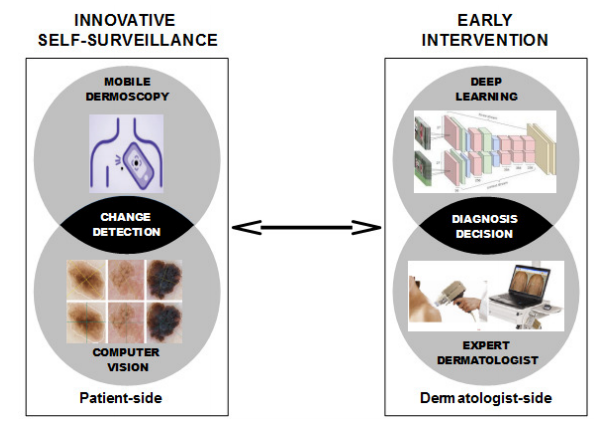
\includegraphics[scale=1,width=\linewidth]{figures/Dissertation_Plan.png}
  \caption{Proposed eHealth application diagram}
\end{figure}
\section{Conclusion}
As the incidence of skin cancer rises, there is a clear need for skin lesion diagnosis tools integrated within eHealth applications that provide support for patients and health professionals. At the same time, new advancements on deep learning methods allow near dermatologist performance with high margin for improvement which overshadow other methods. Challenges such as the requirement for large datasets or the high computational requirements hamper the performance of models and need to be addressed before deploying such tools into production. However, promising techniques such as transfer learning and data augmentation prove to minimize the effects of such factors. Finally, it is expected that these issues will become less relevant as more labeled skin lesion data becomes publicly available.



% conference papers do not normally have an appendix

% trigger a \newpage just before the given reference
% number - used to balance the columns on the last page
% adjust value as needed - may need to be readjusted if
% the document is modified later
%\IEEEtriggeratref{8}
% The "triggered" command can be changed if desired:
%\IEEEtriggercmd{\enlargethispage{-5in}}

% references section

% can use a bibliography generated by BibTeX as a .bbl file
% BibTeX documentation can be easily obtained at:
% http://mirror.ctan.org/biblio/bibtex/contrib/doc/
% The IEEEtran BibTeX style support page is at:
% http://www.michaelshell.org/tex/ieeetran/bibtex/
%\bibliographystyle{IEEEtran}
% argument is your BibTeX string definitions and bibliography database(s)
%\bibliography{IEEEabrv,../bib/paper}
%
% <OR> manually copy in the resultant .bbl file
% set second argument of \begin to the number of references
% (used to reserve space for the reference number labels box)

\bibliographystyle{IEEEtran}
\bibliography{Dissertation.bib}
% that's all folks
\end{document}


